
\chapter{Conclusion} \label{chp:conclusion}

This thesis presents a novel compiler optimisation for reducing code size by merging functions.
Chapter~\ref{chp:fm-operation} describes our novel approach, based on sequence alignment, for merging any two functions.
Chapter~\ref{chp:opt-strategy} describes how our function merging technique can be combined with a optimisation strategy in order to search for profitable functions to merge, which includes a profitability cost model and a ranking of candidate functions.

This chapter is structured as follows:
Section~\ref{sec:conclusion:contribution} summarises the main contributions of this thesis,
%Section 7.2 presents a critical analysis of this work,
Section~\ref{sec:conclusion:futurework} describes future research directions,
and finally Section~\ref{sec:conclusion:summary}  provides concluding remarks.


% We have presented {\ProjName}, a novel compiler-based function merging technique with full support for the SSA form.
% Unlike the previous state-of-the-art, which has to apply register demotion to eliminate the commonly used \textit{phi-nodes} in SSA,
% {\ProjName} directly processes \textit{phi-nodes} using a more powerful code generator.
% As a result, {\ProjName} avoids the code bloating problem introduced by register demotion and
% increases the chances of generating profitable merged functions. We have implemented {\ProjName} in LLVM and evaluated it on the SPEC CPU2006
% and CPU2017 benchmark suites. {\ProjName} delivers on average 9.5\% code reduction for the lowest exploration threshold. Compared to the previous
% function merging state-of-the-art, {\ProjName} achieves $2\times$ more reduction on binary size with 3$\times$ less compile-time overhead and less than half the amount of memory required by it.

% We proposed a novel function merging approach based on sequence alignment, called FMSA. This was the first technique capable of merging any two functions, if deemed profitable, achieving up to 30\% of code-size reduction on SPEC 2006, about twice as much as the past state of the art.
% Although this technique offers significant improvements over previous ones, there are still many limitations and missed opportunities that prevent us from achieving all the available code compression.
% We need to improve the code generator, exploit code reordering, work at different scopes, scale to huge programs, avoid runtime slowdowns, work on JITs, and adopt machine learned heuristics.
% %To address these missed opportunities,
% %We plan to create a better code generator, a new approach that handles code reordering and merges code across different scopes, more accurate cost models
% %, with a better ranking mechanism and code aligner powered by deep learning.
% This will result in smaller programs without runtime or compile time overheads.

\section{Contribution} \label{sec:conclusion:contribution}

This thesis presents a novel function merging technique alongside an optimisation strategy.
Our novel technique uses sequence alignment algorithms from bioinformatics in order to identify the similarity between functions being merged.
The proposed optimisation is very effective at reducing code size by merging arbitrary functions.
Our approach does not suffer from any of the major limitations of existing solutions, outperforming them by more than 2.4$\times$.
We also proposed a ranking-based exploration mechanism to focus the optimization on promising pairs of functions.
Ranking reduces the compilation-time overhead by orders of magnitude compared to an exhaustive quadratic exploration. 
With this framework, our optimization is able to reduce code size by up to 25\%, with an overall average of about 6\%, while introducing an average compilation-time overhead of only 15\%.
Coupled with profiling information, our optimization introduces no statistically significant impact on performance.

\section{Future Work} \label{sec:conclusion:futurework}

For future work, we plan to focus on improving the ranking mechanism to reduce compilation time.
In order to avoid code size degradation, we also plan to improve the compiler's built-in static cost model for code size estimation.
We also plan to work on the linearisation of the candidate functions, allowing instruction reordering to maximize the number of matches between the functions.
Finally, we also plan to incorporate instruction reordering into function merging to maximize the number of matches between the functions regardless of the original code layout.
One can also investigate the application of phi-node coalescing outside function merging.
We envisage further improvements can be achieved by integrating the function-merging optimization to a summary-based  link-time optimization framework, such as ThinLTO in LLVM.
As a future work, we can also analyze the interaction between function merging and other optimizations such as inlining, outlining, and code splitting.

\subsection{Better Code Generator}

%FMSA's code generator is responsible for producing the actual merged functions from the aligned sequences.
%In its original version, FMSA has many artificial limitations in order to simplify its code generator.
%Preliminary results show that the code generator can be significantly improved, enabling far more code compression while reducing compilation time overhead.
%For this project, we plan to develop a new code generator that is capable of appropriately handling $\phi$-nodes, variable length arguments, calling convention, and exploiting target specific instructions to better compress code.
%There are still many opportunities to optimize operand selection and branch instructions that result from merging code. 

In order to better compress code, one can improve the code generator, optimising the parameters used as function identifiers based on calling conventions, exploit target specific instructions, and optimize operand selection and branch instructions that result from merging code.
There are also many missing features in the code generator that are important for its application in the industry.
For example, a new code generator could also be able to appropriately handle variable length arguments, and debug information.
When merging functions, having an optimised code generator is as important as optimally identifying which instructions to merge.
%In the industry, it is also crucial that we appropriately handle debug information when generating code. %link with: \phi$-nodes, variable length arguments
%Appropriately generating code with debug information is crucial for its application in the industry.

\subsection{Handling Code Reordering}

All existing function merging techniques rely on the order in which instructions appear inside the basic blocks and their arrangement,
failing to profitably merge equivalent functions when confronted even with the smallest variations on the ordering of instructions and basic blocks.
Figure~\ref{fig:code-reordering} shows an example of two functions that all existing techniques fail to merge even though they are obviously identical.
Our current technique produces the merged function shown in Figure~\ref{fig:merged-code-reordering}, which is considered unprofitable as it is unable to reduce code size.
Note that all indexing computation is duplicated, including the increment operation, resulting in a merged function that is unnecessarily bigger than the two original functions together.
We need more powerful graph, rather than sequence, alignment techniques to better identify and merge differently ordered but semantically equivalent code.

\begin{figure}[h]
 \centering
 \begin{subfigure}{.5\textwidth}
         \centering
         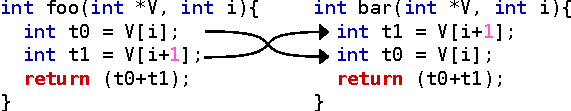
\includegraphics[scale=0.85]{src/conclusion/figs/motivation-1-code.pdf}
         \vspace{1ex}
         \caption{Two equivalent functions.}
         \label{fig:code-reordering}
 \end{subfigure}\begin{subfigure}{.5\textwidth}
         \centering
         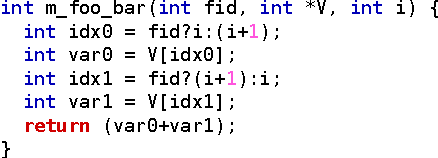
\includegraphics[scale=0.85]{src/conclusion/figs/motivation-1-merged-code.pdf}
         \caption{Merged function currently produced by FMSA.}
         \label{fig:merged-code-reordering}
 \end{subfigure}
    \vspace{-2ex}
    \caption{Example of how even trivial reordering is poorly handled by the existing solutions.}
    \label{fig:code-reordering-example}
\end{figure}

\subsection{Merging Across All Scopes}

Existing techniques are limited to one particular scope.
While function merging is applied only to whole functions,
function outlining is commonly applied at the basic block level.
%In one end we have an optimization such as the function outlining which is capable of merging or extracting equivalent basic blocks, in the other end we have function merging capable of merging whole functions.
However, equivalent code can be found within or across functions, which themselves may reside in the same source file or be spread across multiple source files.
Therefore, we need to develop a novel unified optimization capable of merging semantically equivalent code that can span anything between a single basic block up to a whole function.
This unification has the extra benefit of also addressing the phase ordering problem by coordinating the merge operations on different scopes.

\subsection{Scaling for Large Programs}

Although our optimisation achieves very good results in terms of code compression, it is still unable to handle large programs in a real scenario.
Its time complexity and memory usage requirements would prevent it from optimizing large programs such as web browsers, Clang/LLVM, and operating systems, as these programs tend to have many functions with several thousands of instructions.
Link-time optimization (LTO) makes this matter even worse by optimizing the code after the whole program has been linked into a single module, imposing a huge pressure on memory usage and compilation time.

%In this project, we will investigate this scalability issue.
%We plan to perform link-time optimization in an incremental fashion, such as using ThinLTO, which operates on individual translation units, reducing memory usage while also making it suitable for parallel and distributed compilation.
The optimization of different translation units can be distributed across different machines and merge operations locally performed in parallel.
In order for this to work, an important challenge that needs to be addressed concerns ranking and merging functions that reside in different translation units.
However, this is essential to enable the use of LTO on real programs while keeping the memory usage and compilation time acceptable.

\subsection{Powered by Deep Learning}

In order to reduce compilation time while also being effective, 
the ranking-based exploration mechanism tries to efficiently focus the search 
only to the most promising pairs of functions.
However, the existing solution is still very wasteful as most of the merged functions are
discarded by the profitability analysis.
Identifying what would be profitably merged is a very challenging task.

Given our group's expertise on the area, we plan to use solutions based on deep learning to efficiently predict which pairs of functions are most likely to be profitable to merge.
This approach has the potential to reduce compilation time even further while also improving the compression by finding profitable candidates that are currently missed.
Having accurate target-specific cost models is crucial for the effectiveness of the profitability analysis.
We plan to explore the use of machine learning techniques to develop more accurate cost models.

One can investigate the use of deep learning to align two functions and better identifying what can be merged.
Sequence alignment focusses only on maximizing the number of merged instructions,
without necessarily minimizing the number of operand selections or branches.
A smarter approach that understands how instructions interact with each other would be
very beneficial.


\subsection{Avoiding Performance Overheads}

For many real applications, it is desirable to achieve a good balance between code size and performance.
Preliminary results show that performance degradation can be completely avoided by using profiling to
guide the merging decisions.
One can avoid adding branches inside hot execution paths, therefore avoiding performance penalties.
Although hot code can be merged, it is important to minimize unnecessary branches when merging hot code.
We will develop a profile-guided optimization that automatically identify the best trade-off between code-size and performance.

\subsection{Less Memory Usage by JIT}

Ahead-of-time and just-in-time (JIT) compilation have completely different requirements.
Function merging can be used to reduce the amount of memory used by programs running on a JIT environment.
However, our solution must be adapted to the requirements that are specific to a JIT environment, as JIT compilers have the extra challenge of having to optimize the code as fast as possible.
This would require the development of completely new algorithms for ranking and aligning functions that are suitable for this application domain.
Another possibility is to exploit the fact multiple programs may be simultaneously running on the same JIT environment and merge code across different programs, reducing the overall memory usage.

\section{Summary} \label{sec:conclusion:summary}